% Apendice
\chapter{Informaci'on adicional de {\tt d2Hgr}}

\begin{figure}[htb]
\centering
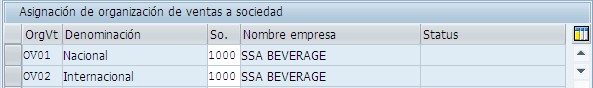
\includegraphics[scale=0.65,type=jpg,ext=.jpg,read=.jpg]{figures/OrgVentasSociedad}
\caption{Asignaci'on de las Organizaciones de Ventas a la Sociedad}
\label{fig:asigna1}
\end{figure}
\begin{figure}[htb]
\centering
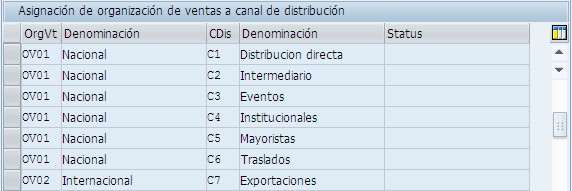
\includegraphics[scale=0.65,type=jpg,ext=.jpg,read=.jpg]{figures/OrgVentasCanales}
\caption{Asignaci'on de las Organizaciones de Ventas a los Canales de Distribuci'on}
\label{fig:asigna2}
\end{figure}
\begin{figure}[htb]
\centering
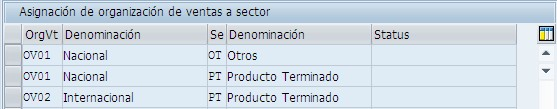
\includegraphics[scale=0.65,type=jpg,ext=.jpg,read=.jpg]{figures/OrgVentasSector}
\caption{Asignaci'on de las Organizaciones de Ventas a los Sectores}
\label{fig:asigna3}
\end{figure}
\begin{figure}[htb]
\centering
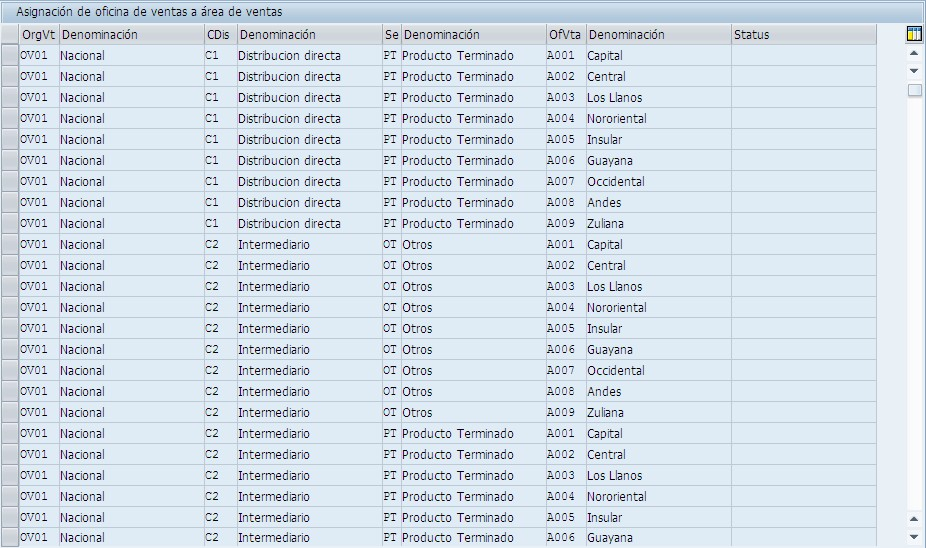
\includegraphics[scale=0.65,type=jpg,ext=.jpg,read=.jpg]{figures/OfVentaAreas}
\caption{Parte de la asignaci'on de las Oficinas de Ventas a las 'Areas de Ventas}
\label{fig:asigna4}
\end{figure}
\begin{figure}[htb]
\centering
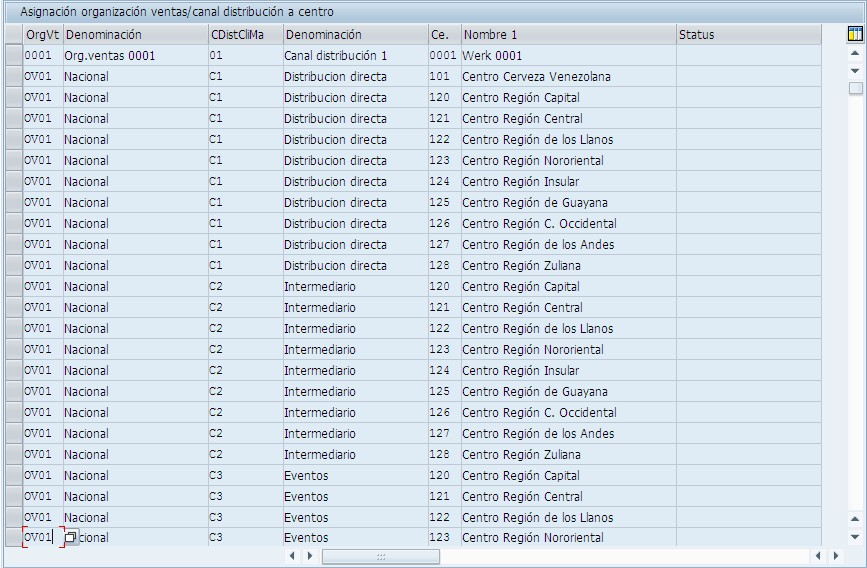
\includegraphics[scale=0.65,type=jpg,ext=.jpg,read=.jpg]{figures/OrgCanalCentro}
\caption{Parte de la asignaci'on de las Orgnanizaciones de Ventas y Canales de Distribuci'on a los Centros de Distribuci'on}
\label{fig:asigna5}
\end{figure}
\begin{figure}[htb]
\centering
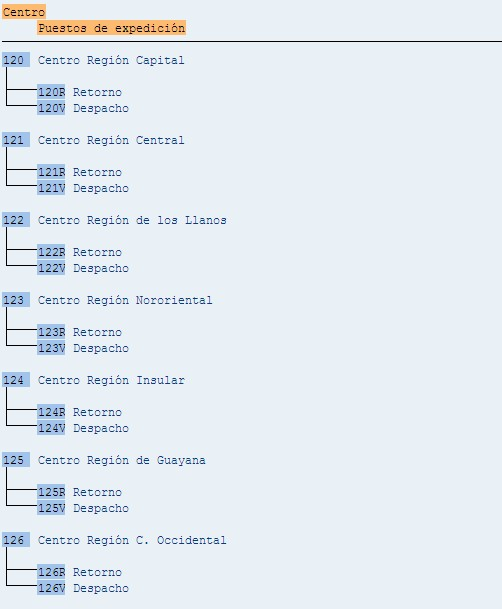
\includegraphics[scale=0.65,type=jpg,ext=.jpg,read=.jpg]{figures/ExpedicionCentro}
\caption{Parte de la asignaci'on de los Puestos de Expedici'on a los Centros de Distribuci'on}
\label{fig:asigna6}
\end{figure}

AQU\'I VA EL CONTENIDO DE LOS AP\'ENDICES.
%Puedes quitar esto(es opcional)
\vspace{5 mm}

Esta parte del ap'endice contiene el manual del usuario de la herramienta
implementada, la descripci'on de sus archivos y el c'odigo fuente de algunos
m'odulos de posible inter'es.

\section{Requerimientos de {\it software} y {\it hardware}}
\label{sect:hardsoftrequirements}

El programa resultante deber'ia poder ser utilizado sobre cualquier maquina 
con m'as de 32 MB libres de RAM. Aunque no hay limitaciones para el procesador
a usar, entre m'as nuevo el procesador y mayor n'umero de n'ucleos tenga, m'as
r'apido har'a los calculos la herramienta. En el caso de la memoria, entre 
m'as tenga disponible la herramienta, mayor cantidad de datos podr'a utilizar 
en los c'alculos.

\begin{itemize}
\item Para su compilaci'on, el programa requiere una versi'on actualizada de
gcc, el compilador {\tt C} GNU. Se ha utilizado varias versiones para su
compilaci'on por lo cualquier versi'on mayor a la $4.2$ deber'ia funcionar.
\item La liber'ia {\tt libpcap} es necesaria para darle las funcionalidades de
manipulaci'on de trazas {\tt tcpdump} al programa. A partir de la versi'on
$0.8$ se encuentran todas las funciones que utiliza el programa.
\item La compilaci'on de la herramienta se hace m'as f'acil con {\tt make},
programa GNU. Cualquier versi'on mayor a $3.6$ no deber'ia dar problemas.
\item El programa {\tt gnuplot} es indispensable para poder graficar los
resultados creados por el programa. La versi'on m'as utilizada durante su
desarrollo fue la $4.2$ por lo que es la que se recomienda.
\item La graficaci'on s'olo se puede hacer sobre un sistema operativo bajo el
est'andar POSIX\footnote{"Portable Operating System Interface [for Unix]" son
una familia de est'andares de llamadas al sistema operativo definidos por la
IEEE y especificados formalmente en el IEEE 1003. La gran mayor'ia de las
distribuciones GNU/Linux siguen los est'andares aunque no est'an
oficialmente certificados.} con la herramienta gnuplot instalada. Esto se debe
a una necesidad de la interfaz gnuplot en ANSI C que utiliza un ``pipe'' tipo
POSIX para comunicarse directamente con el programa gnuplot instalado en la
m'aquina. Sin embargo, dentro de las opciones del programa se puede pasar la
informaci'on obtenida en la estimaci'on a archivos de texto para su posterior
an'alisis.
\item La librer'ia pthreads da las funciones necesarias para utilizar hilos
de ejecuci'on en el programa.
\end{itemize}

\section{Ayuda de la l'inea de comando} \label{sect:ayuda}

La herramienta toma como par'ametro principal un archivo {\tt tcpdump} o un CSV
de una serie de tiempo pseudo-aleatoria generada con la herramienta R.
Aparte se puede escoger una velocidad de captura, una ventana, una ventana
deslizante, filtrar paquetes, delimitar corridas, correr con varios hilos de
ejecuci'on, adem'as de estimar el par'ametro de Hurst con los tres m'etodos
mencionados. Se puede tambi'en obtener el cambio del par'ametro de Hurst en el
tiempo o graficar la estimaci'on de una ventana en particular. La ayuda de la
l'inea de comando se muestra abajo:

\begin{alltt}
\label{verb:help}
Usage: ./d2Hgr -[f|g] file -[i|nrlvxmu] [OPTIONS]                               

Estimate and graph Hurst parameter calculations from a file.

   -f file   Specifies a tcpdump dump file.
   -g file   Specifies a CSV file with a simulated network traffic stream.
             This option cannot be used with the time based or tcpdump
             options since the stream is simulated and is static in it's
             definition.
   -i        Prints only the protocol statistic information available from the
             tcpdump file.
   -n        Tells the program if you wish to graph the packets per delta time
             graph. Affected by -p, -o, -d, -c, -b -e, -y flags.
   -r        Tells the program to calculate the Hurst parameter changes over
             time by use of the R/S statistic. Affected by -p, -o, -d, -c, -w,
             -s, -j, -t, -b, -e, -y flags.
   -l num    Tells the program to graph the Pox diagram that creates the Hurst
             data point for a given window number between 0 and Datapoints
             designated by num. Affected by -p, -o, -d, -c, -w, -s, -j, -b,
             -e, -y flags.
   -v        Tells the program to calculate the Hurst parameter changes over
             time by using the Variance-time plot technique. Affected by -p,
             -o, -d, -w, -s, -j, -t, -b, -e, -y flags.
   -x num    Tells the program to graph the Variance-time plot that estimates
             the Hurst parameter for a given window number designated by num.
             Affected by -p, -o, -d, -c, -w, -s, -j, -b, -e, -y flags.
   -m        Tells the program to calculate the Hurst parameter changes over
             time by use of the Modified Allan Variance. Affected by -p, -o,
             -d, -c, -w, -s, -j, -t, -b, -e, -y flags.
   -u num    Tells the program to graph the Modified Allan Variance that
             estimates the Hurst parameter for a given window number designated
             by num. Affected by -p, -o, -d, -c, -w, -s, -j, -t, -b, -e, -y
             flags.

 OPTIONS:
   -p proto  Specifies which protocol to be taken into account when doing
             calculations. Default is all.
             Implemented protocols are:
              ip tcp udp icmp sctp ftp ssh telnet smtp dns dhcp http pop3 ntp
              imap snmp ldap https smtps ldaps imaps pop3s nfs squid
   -o dir    Output directory for results. Default is current directory.
   -d        Tells the program if the results should be placed in text files
             for later use. This option doesn't graph. Useful for using this
             program where gnuplot is not available.
   -y        Tells the program to graph and print the resulting data files.
   -a        Tells the program not to graph or create data files.
   -c sec    Specify a packet capture speed. This makes the program not look
             for one. Example: 0.01 = 0.01 seconds.
   -w sec    Window time size. This makes the program not look for one.
             Example: 60 = 60 seconds.
   -s sec    Slide time size. This makes the program not look for one.
             Example: 1 = 1 seconds.
   -j num    Tells the program to use log base num for all the calculations of
             blocks for the R/S statistic, Variance-time plot and Modified Allan
             Variance. Default is 2.
   -t num    Does Hurst calculation using threads. If 0 is placed, then the
             default number of threads (4) is used.
   -b sec    Tells the program from which second in the time data to begin the
             calculation. Default is 0s.
   -e sec    Tells the program how many seconds after the beginning point to
             include in the calculation. Default is the whole tcpdump time.
   -k num    Average Hurst parameter change with which to try to detect attacks.
   -K num    Standard deviation of Hurst parameter change with which to detect
             attacks.
   -q num    Average Hurst parameter value with which to try to detect attacks.
   -Q num    Standard deviation of Hurst parameter value with which to detect
             attacks.
   -h        Print this help.
\end{alltt}

\section{Archivos del programa}

El programa de C llamado {\tt d2Hgr}, consiste de 18 archivos de c'odigo fuente
que incluye 9 archivos de cabecera. Los archivos contienen la siguiente
informaci'on:

\begin{itemize}
\item{\bf config.h}: Cabecera de funciones para parsear las opciones de linea
de comando.
\item{\bf config.c}: Implementaci'on de las funciones que parsean las opciones
de la linea de comando.
\item{\bf d2Hgr.h}: Archivo que contiene las definiciones de las funciones para
leer los archivos producidos por {\tt tcpdump}.
\item{\bf d2Hgr.c}: Implementaci'on de las funciones para leer la informaci'on
del archivo producido por {\tt tcpdump} y poder obtener la informaci'on
necesaria para su posterior an'alisis.
\item{\bf externvars.h}: Archivo que contiene todas las estructuras especiales
para el uso del programa.
\item{\bf filter.h}: Archivo que contiene la definici'on de las funciones para
construir la expresi'on de filtro de libpcap para usar durante la corrida del
programa.
\item{\bf filter.c}: Archivo que contiene la implementaci'on de todas las
funciones de filter.h.
\item{\bf flows.h}: Cabecera de funciones para contabilizar los flujos de IPv4.
\item{\bf flows.c}: Archivo que contiene la definici'on de las funciones para
contabilizar los flujos de IPv4.
\item{\bf gnuplot\_i.h}: Cabecera para el archivo gnuplot\_i.c que define las
funciones de la interfaz gnuplot para que el programa pueda graficar los
resultados. Esta es una versi'on modificada de la interfaz ANSI C de N.
Devillard para gnuplot.
\item{\bf gnuplot\_i.c}: Implementaci'on de las funciones de N. Devillard para
su interfaz de ANSI C con gnuplot.
\item{\bf graph.h}: Archivo que contiene la definici'on de las funciones para
graficar los resultados.
\item{\bf graph.c}: Archivo que contiene la implementaci'on de las funciones
para graficar los resultados.
\item{\bf hurst.h}: Archivo que contiene las definiciones de los m'etodos para
aproximar el par'ametro de Hurst.
\item{\bf hurst.c}: Archivos que contiene las implementaciones de los m'etodos
para aproximar el par'ametro de Hurst y los m'etodos para extraer la
informaci'on sobre los paquetes una vez leidos por las funciones de d2Hgr.h.
\item{\bf main.c}: El archivo que contiene el main del programa.
\item{\bf detect.h}: El archivo que contiene las definiciones de los m'etodos 
para la detecci'on de ataques de denegaci'on de servicio.
\item{\bf detect.c}: El archivo que contiene las implementaciones de los 
m'etodos para la detecci'on de ataques de denegaci'on de servicio.
\end{itemize}

\section{Creaci'on de $Xtdata$}

\lstinputlisting[caption={Creaci'on de $Xtdata$},label={cod:xtdata}]{code/xtdatacreate.c}


